\documentclass{article}
\usepackage[a4paper, total={6.6in, 9in}]{geometry}
\usepackage{amsmath}
\usepackage{amssymb}
\usepackage{authblk}
\usepackage{bbm}
\usepackage{booktabs}
\usepackage{diagbox}
\usepackage{graphicx}
\usepackage{listings}
\usepackage{multirow}
\usepackage{xcolor}
\usepackage[colorlinks=true,
    linkcolor=blue, 
    urlcolor=blue, 
    citecolor=blue, 
    anchorcolor=blue]{hyperref}
%\usepackage{slashbox}
\allowdisplaybreaks

\title{CSCI-SHU 360 Machine Learning\\
    Report of Final Competition}
\author{Yufeng \textsc{-AeoLian-} Xu  \texttt{yx3038@nyu.edu}}

\begin{document}
    \maketitle

    \section{Guideline}
    This section aims to provide a navigation of this repository. 
    \begin{itemize}
        \item Folder \texttt{src} contains the source code of the final competition.
        \item File \texttt{main.py} is the main file for training of the models. File \texttt{data\_utils.py} contains the functions for data processing as well as the customized dataset class. File \texttt{models.py} contains the customized ResNet18. File \texttt{infer.py} utilizes the ensemble of several trained model to make predictions.
        \item Folder \texttt{write-up} contains the report on the final competition.
        \item Folder \texttt{checkpoints} records the parameters, prediction, as well as best validation accurcay so far for each of the models.
        \item Folder \texttt{data} contains the original as well as processed data.
        \item File \texttt{prediction.csv} is the prediction made by \texttt{infer.py}.
    \end{itemize}

    \section{Data Preprocessing}
    We called a Python library called \texttt{spleeter} to separate vocal and instrumental parts in each music snippet, and chose and vocal parts as our training and evaluation  data. Afterwards, we used \texttt{torchaudio} to load and transform(or augment) the vocal files.

    \section{Models}
    \subsection*{Architecture}
    The models I have tried for the final competition include: ResNet18, ResNet50, ResNet101, ResNext, Dense-Net201, Vision Transformer (ViT), Long Short Term Memory (LSTM).
    Among all these models, ResNet18 demonstrates excellent performance and the best performance-efficiency tradeoff. Therefore, the final results are based on resnet18. An unexpected observation is that the resnet18 network implemented by myself has better performance than the built-in one from torch, although according to \textbf{model.modules} the two have exactly the same components.\\
    The architecture of my ResNet18 model is shown in Figure 1.
    \begin{figure}[hbt!]
        \centering
        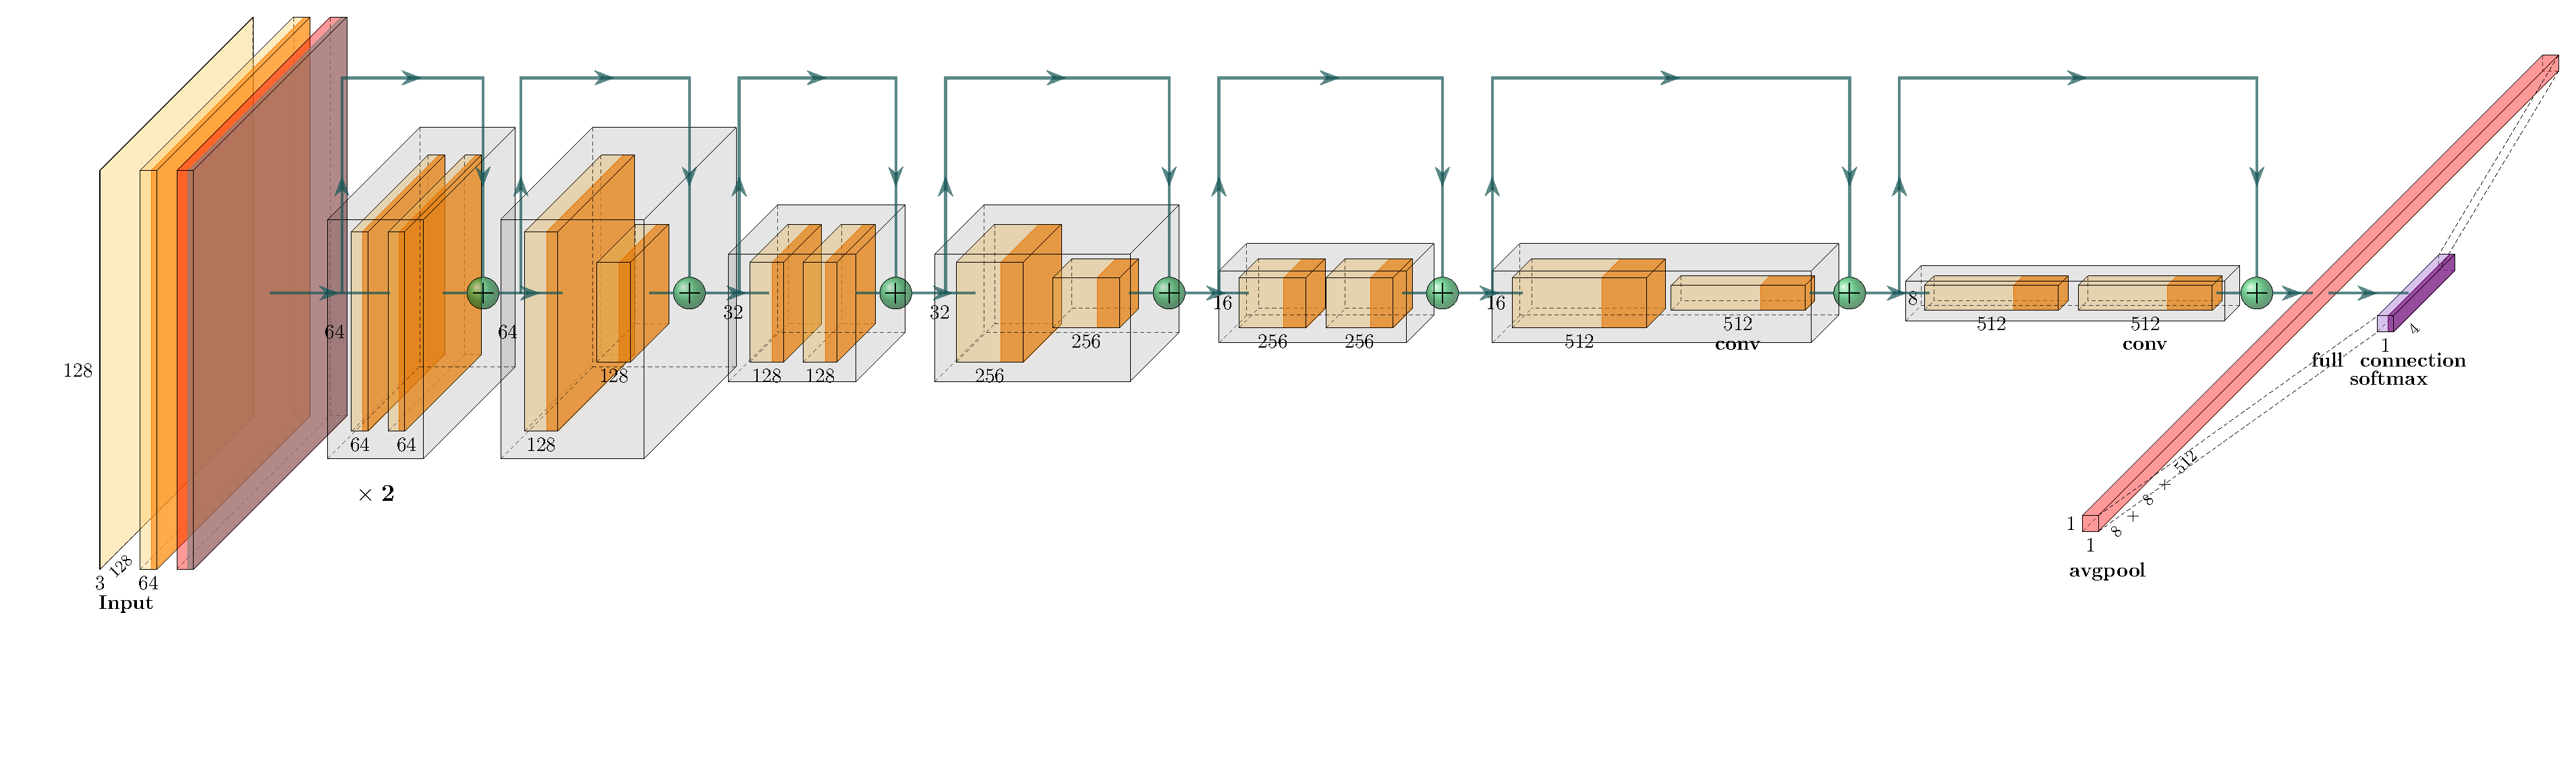
\includegraphics[width=1\textwidth]{../PlotNeuralNet/my_arch/arch.pdf}
        \caption{The architecture of my ResNet18 neural network. Only convolutional layers, pooling layers, and fully connected layers are illustrated; batch norm layer and ReLU function are applied after each convolutional layer, and they are omitted from the chart.}
    \end{figure}

    \subsection*{Computational Consumption}
    Most of the code was run on NYU Greene HPC RTX8000 GPU, on which an epoch takes 2 minutes on average. The final submission is based on an ensemble of 8 resnet18 models, and each model is trained for 24 epochs, so the total estimated running time is 384 minutes$\approx$6 hours.

    \newpage{}
    \section{Training Setups}

    \subsection*{Vocal Separation}
    We applied a pretrained Python library called spleeter to separate the vocal part and instrumental part in each of the music snippet. The mode of the separator is "spleeter:2stems". The detailed code can be found in \texttt{src/data\_utils.py}.

    \subsection*{Data Transformatation}
    The audio data is loaded by \texttt{torchaudio}, and converted to Mel spectrograms, and processed with an amplitude-to-db transform. \\
    Considering the dataset is class-imbalanced and the number of samples with label 0 is approximately the number of samples with other labels, we append 3 copies of samples of label 0 to the dataset.\\
    Afterwards, the data is copied and the copy goes through an i.i.d. random time masking, so that the dataset has more diversity.\\
    Also, we applied mixup augmentation to the training data, which can be formualted as $x'=\lambda\cdot x_1+(1-\lambda)\cdot x_2$, where $\lambda$ is sampled from a $\beta$-distribution $B(0.2,0.2)$.\\
    Lastly, the data is splitted into a train set and a validation set with \texttt{test size=0.2, random state=42}.

    \subsection*{Optimization}
    The model is optimized with stochastic gradient descent (SGD) with \texttt{lr=1e-3}, \texttt{momentum=0.9},\texttt{weight\_decay=0}. Each of the models was trained for 24 epoch with the learning rate annealed by 10 every 6 epochs.\\
    I also tried cosine learning rate annealing, as well as cosine annealing with warm restart, but they did not provide results better than multi-step annealing, so multi-step annealing is the final scheduler.

    \section{Results}
    The plot of the metrics during training I obtained from \texttt{wandb} are shown in Figure 2.\\
    It is worth noting that mixup augmentation significantly increases the final value of convergence of the loss function, but the validation accurcay is slightly improved with this augmentation.\\
    The final accuracy on test set is 79.56\% (as shown on the Kaggle leaderboard). If you want to reproduce this result, you can simply run \texttt{src/infer.py}, which loads the model parameters and generates prediction with ensemble.
    \newpage{}
    \begin{figure}[hbt!]
        \centering
        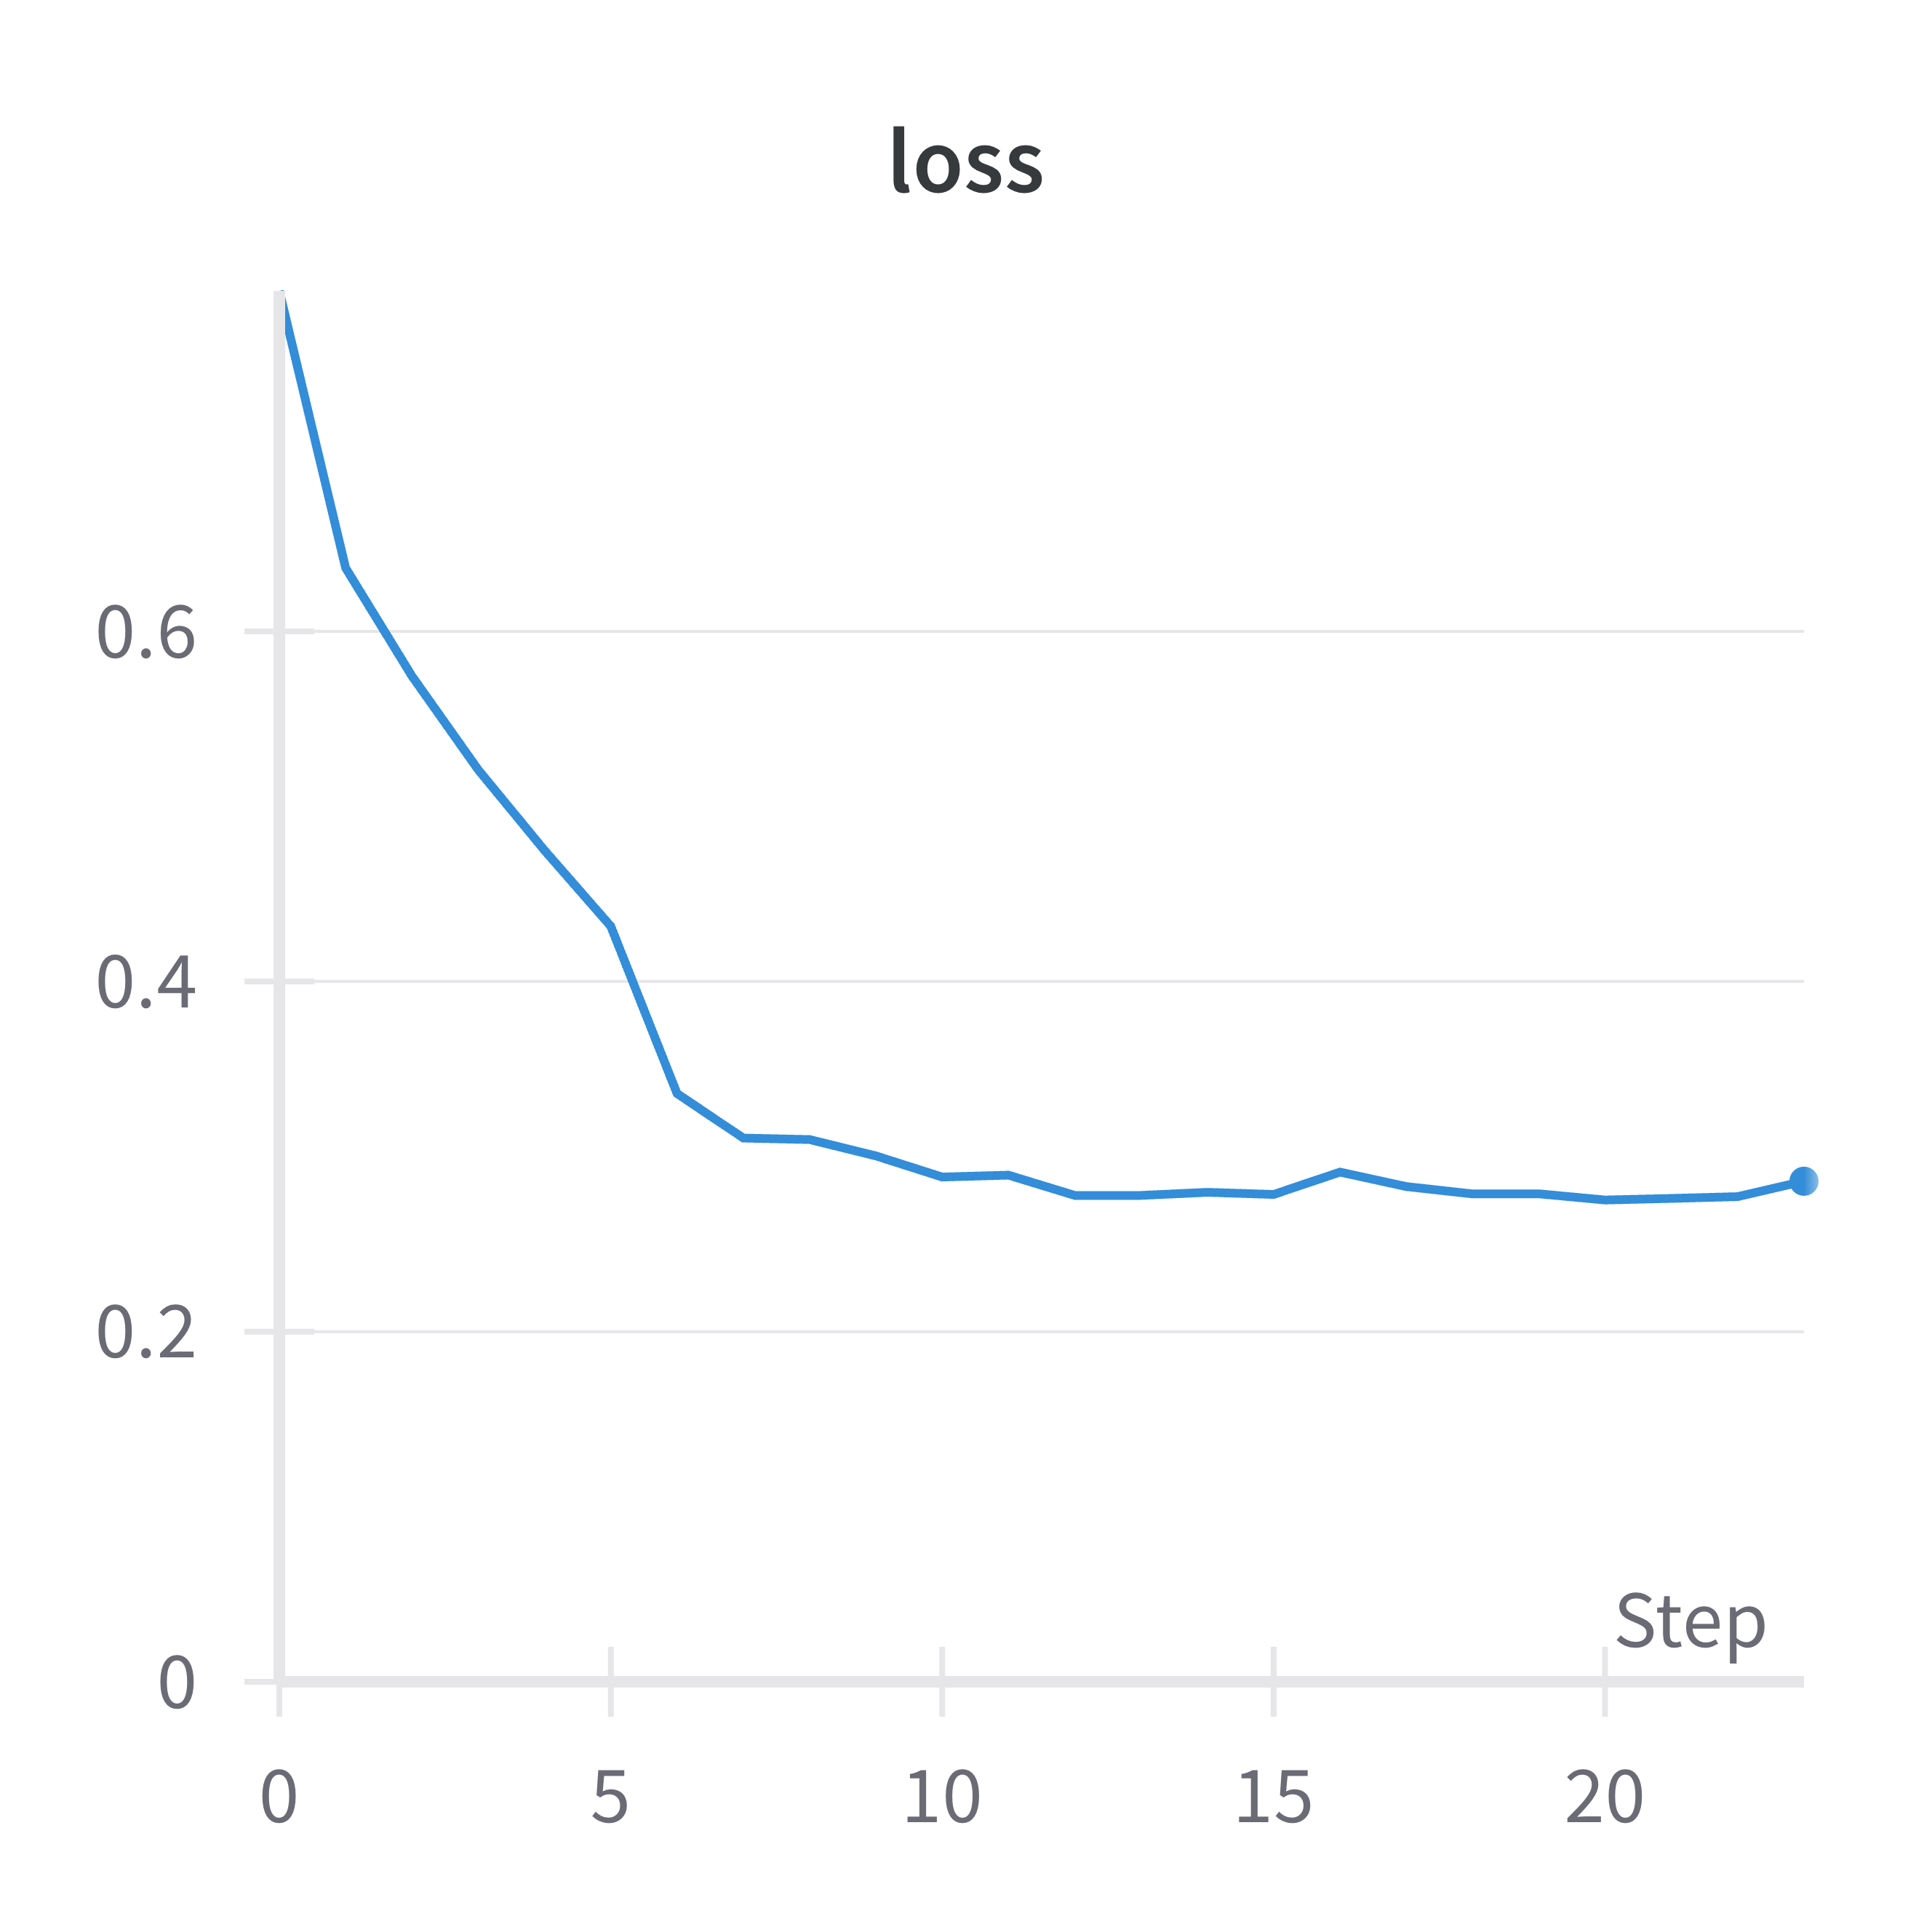
\includegraphics[width=0.3\textwidth]{figs/loss.png}
        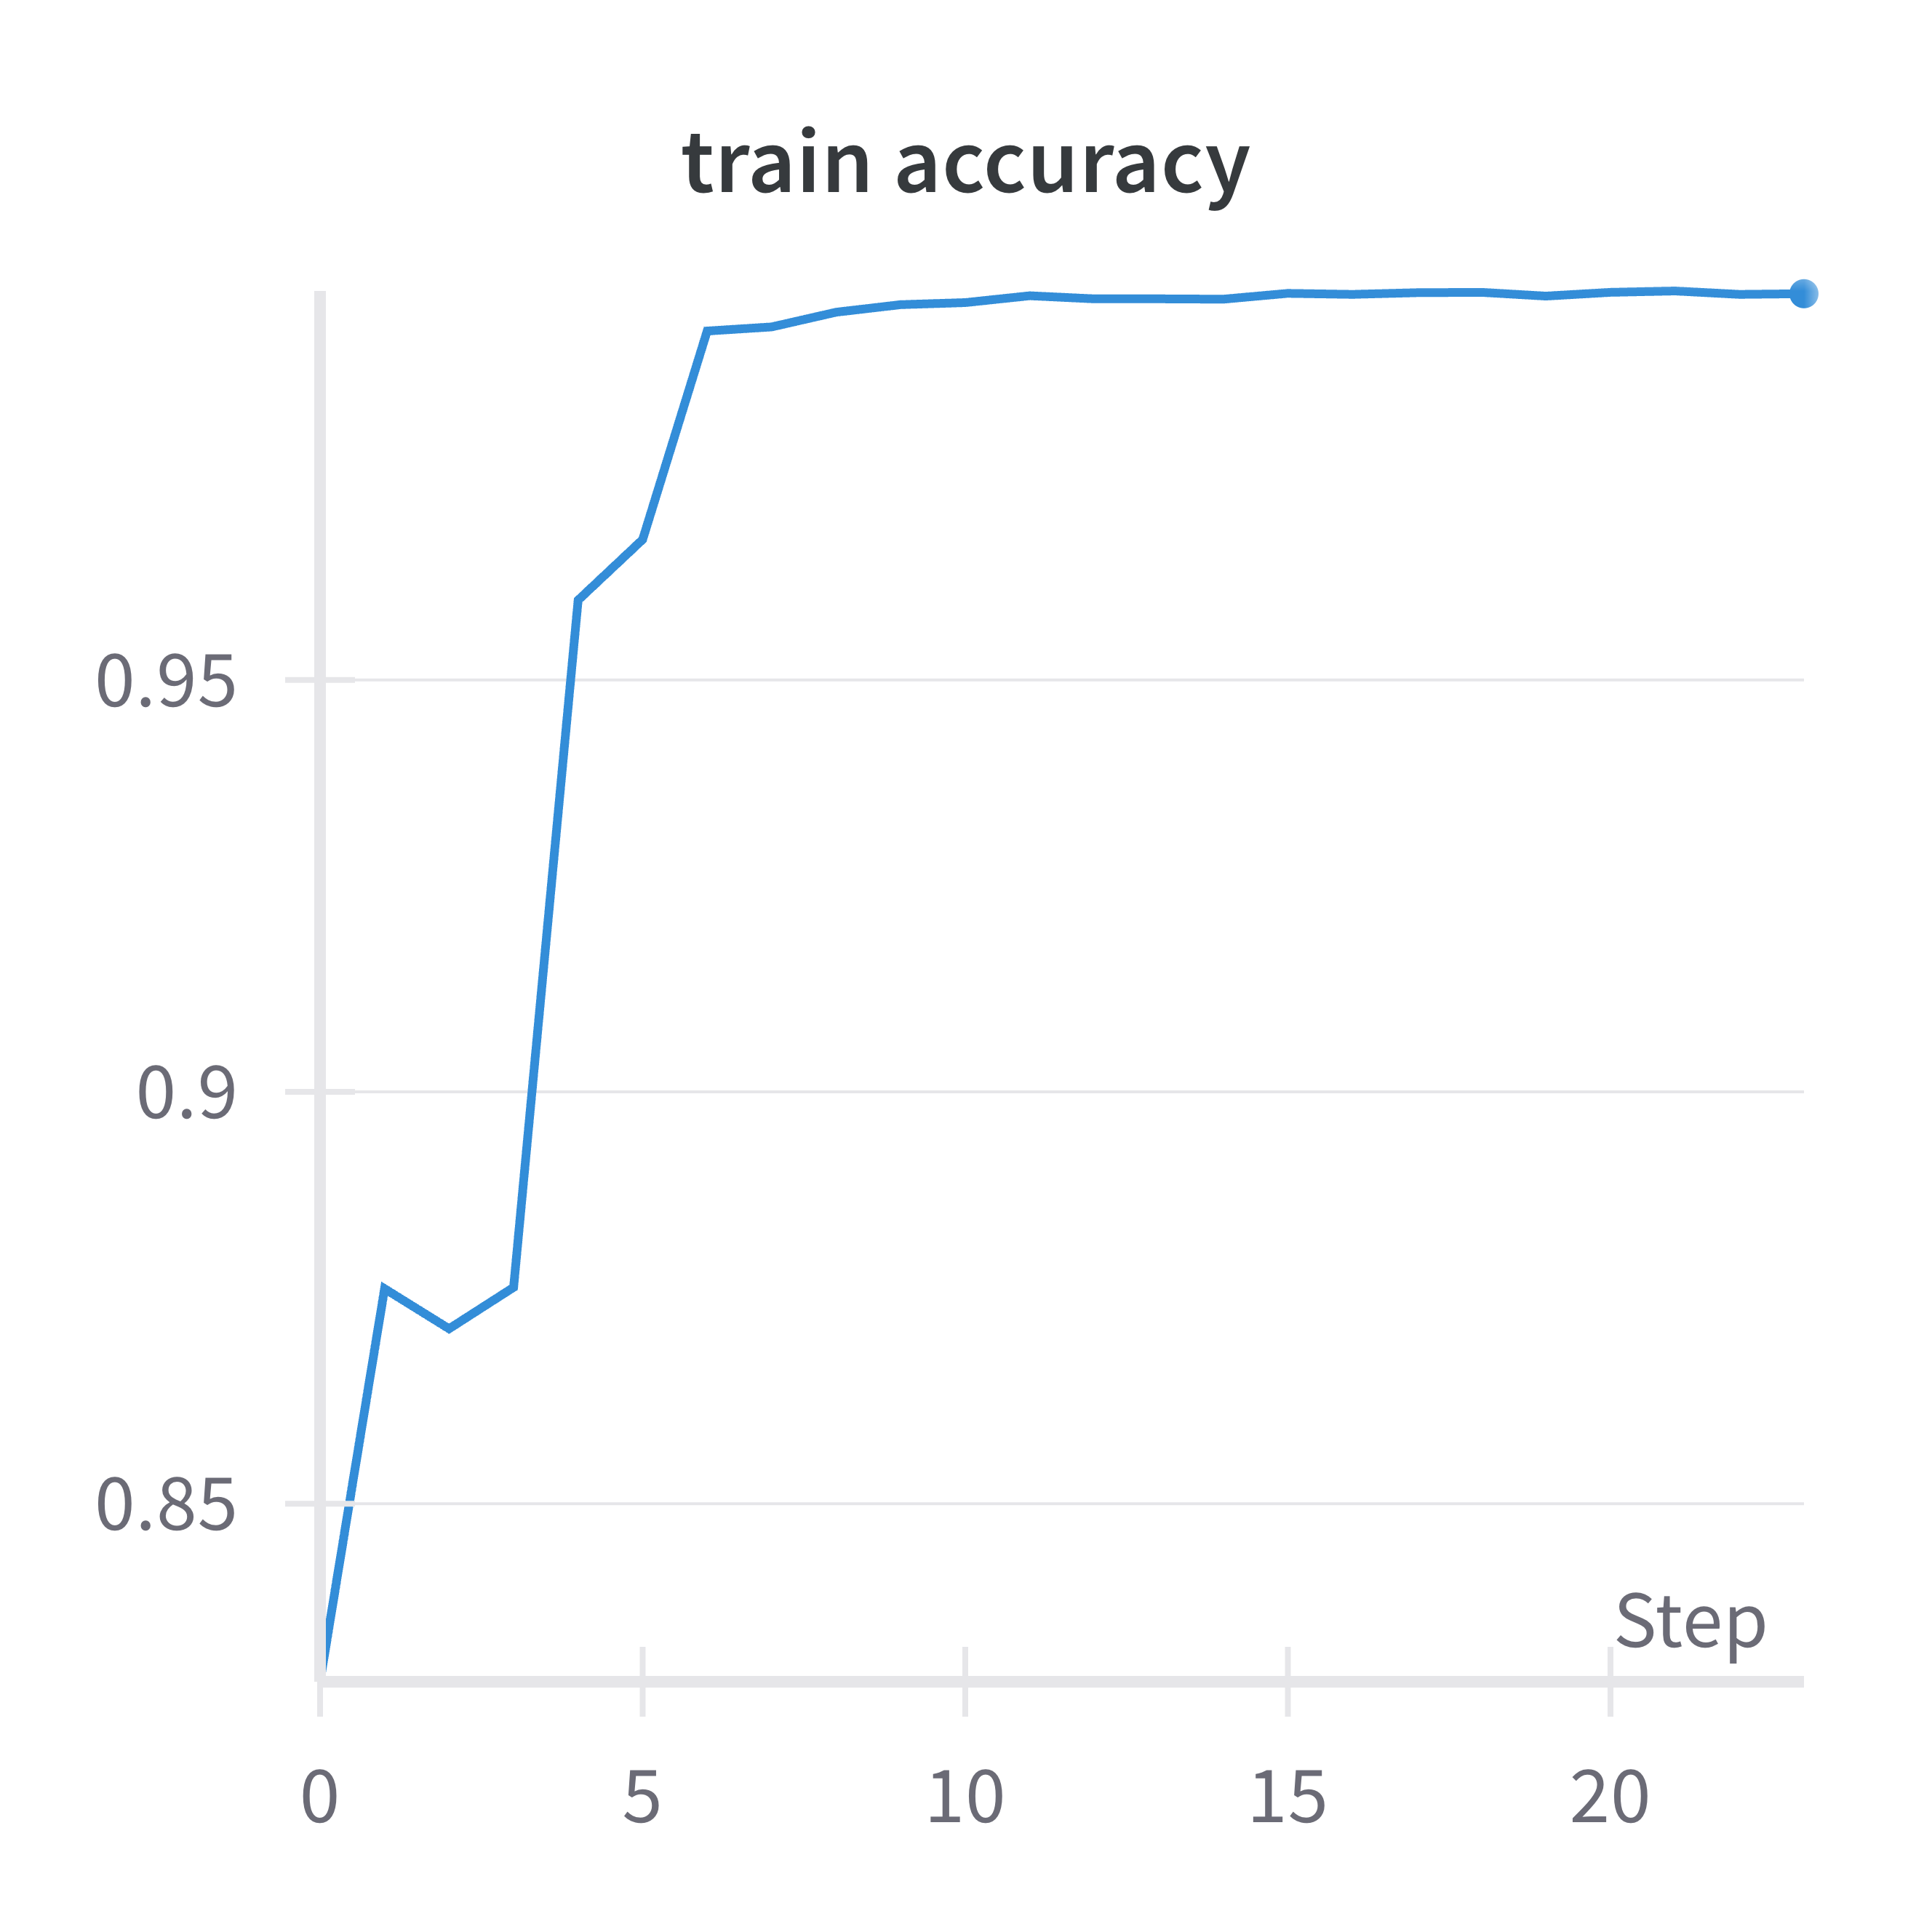
\includegraphics[width=0.3\textwidth]{figs/train.png}
        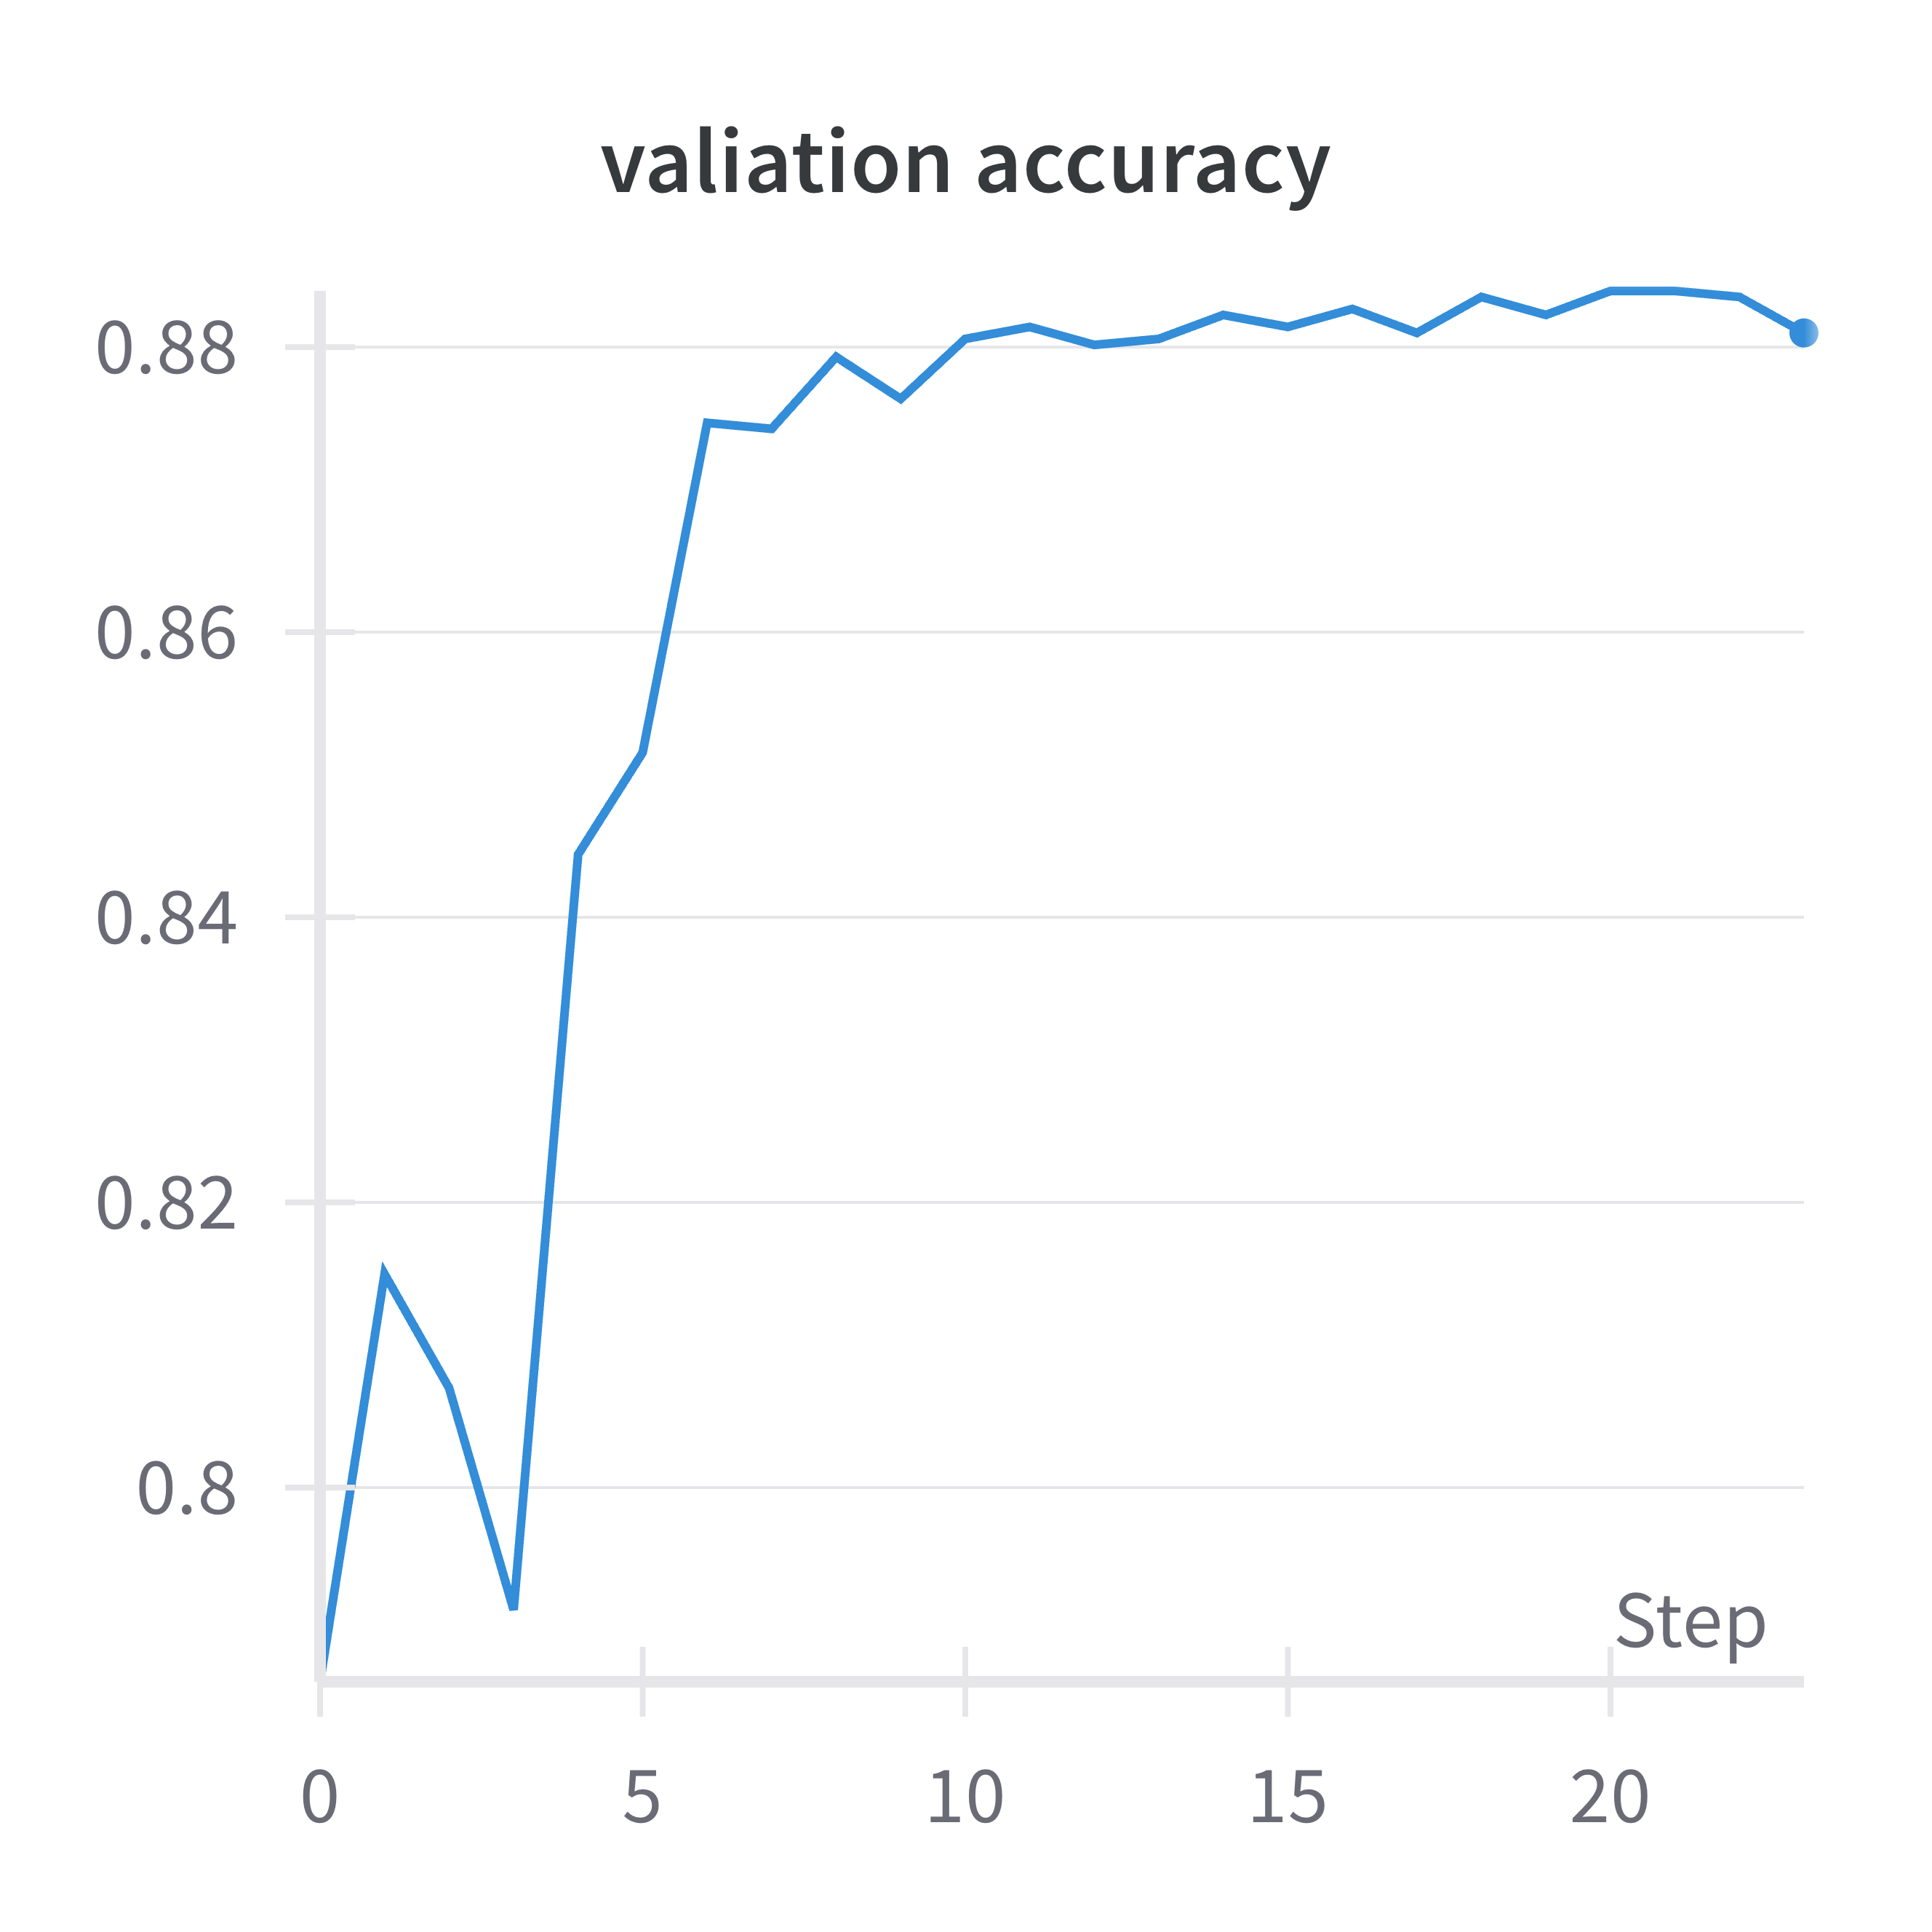
\includegraphics[width=0.3\textwidth]{figs/val.png}
        \caption{The plots of the metric during training obtained from \texttt{wandb}. Left: training loss; middle: train accuracy; right: validation accuracy.}
    \end{figure}



\end{document}